\documentclass[11pt,a4paper]{article}
\usepackage[utf8]{inputenc}
\usepackage[T1]{fontenc}
\usepackage{geometry}
\geometry{margin=1in}
\usepackage{hyperref}
\usepackage{amsmath}
\usepackage{amssymb}
\usepackage{booktabs}
\usepackage{longtable}
\usepackage{graphicx}
\usepackage{xcolor}
\usepackage{listings}
\usepackage{titlesec}
\usepackage{fancyhdr}
\usepackage{enumitem}
\usepackage{mdframed}
\usepackage{tabularx}
\usepackage{array}

% Header and footer
\pagestyle{fancy}
\fancyhf{}
\rhead{\textbf{SoundTag Federated Learning Plan v2.0}}
\lhead{\textcolor{gray}{Confidential}}
\rfoot{\thepage}

% Title formatting
\titleformat{\section}{\Large\bfseries\color{black}}{\thesection}{1em}{}
\titleformat{\subsection}{\large\bfseries}{\thesubsection}{1em}{}
\titleformat{\subsubsection}{\normalsize\bfseries}{\thesubsubsection}{1em}{}

% Highlighted box for key decisions
\newmdenv[
  backgroundcolor=gray!10,
  linecolor=black!40,
  linewidth=1pt,
  roundcorner=4pt,
  innerleftmargin=10pt,
  innerrightmargin=10pt,
  innertopmargin=8pt,
  innerbottommargin=8pt
]{keybox}

% Code listing style
\lstset{
    basicstyle=\ttfamily\small,
    keywordstyle=\color{blue},
    stringstyle=\color{red},
    commentstyle=\color{gray},
    breaklines=true,
    frame=single,
    numbers=left,
    numberstyle=\tiny\color{gray},
    xleftmargin=1.5em,
    framexleftmargin=1.5em
}

\title{%
  \vspace{2cm}
  \Huge\textbf{SoundTag: A Federated Learning Framework} \\
  \vspace{0.4cm}
  \Large for Urban Noise Classification \\
  \vspace{0.5cm}
  \large Technical Design Document --- Version 2.0
}
\author{SoundTag ML Team}
\date{\today}

% ============================================================
\begin{document}
% ============================================================

\maketitle
\thispagestyle{fancy}

\newpage
\tableofcontents
\newpage

% ============================================================
\section{Purpose and Scope}
% ============================================================

This document defines the complete technical framework for training and deploying a
machine learning (ML) model---and subsequently a deep learning (DL) model---for urban
noise classification under the SoundTag project, using \textbf{federated learning (FL)}
as the primary training paradigm.

\begin{keybox}
\textbf{Core objective.} Train noise classification models collaboratively across
edge devices (Android phones, web browsers) without centralising raw audio data.
The model is the primary deliverable. Automatic on-device inference is a secondary
by-product that emerges once the model is trained.
\end{keybox}

\subsection{What this document covers}
\begin{itemize}[leftmargin=*,noitemsep]
  \item Data collection pipeline and JSON schema (source of truth for training)
  \item Feature extraction pipeline (server-side, reproducible, environment-agnostic)
  \item ML Phase: classical models trained on handcrafted features
  \item DL Phase: CNN/CRNN trained end-to-end on mel spectrograms
  \item Federated learning framework: weight exchange, aggregation, round management
  \item Central server architecture and infrastructure
  \item Deployment of trained models back to edge devices (inference as by-product)
\end{itemize}

\subsection{What this document does not cover}
\begin{itemize}[leftmargin=*,noitemsep]
  \item Annotation UI/UX design (handled by the Android/web app teams)
  \item Map visualisation or noise heatmap generation
  \item Real-time streaming inference (post-publication scope)
\end{itemize}

% ============================================================
\section{Existing System: Data Collection Layer}
% ============================================================

\subsection{Client Applications}

The SoundTag project currently operates two data collection clients:

\begin{table}[h]
\centering
\caption{Data Collection Client Summary}
\begin{tabular}{@{}p{3.2cm}p{5cm}p{5cm}@{}}
\toprule
\textbf{Aspect} & \textbf{Android App (Kotlin)} & \textbf{Web App (Next.js/React)} \\
\midrule
Language & Kotlin & TypeScript / JavaScript \\
Framework & Jetpack Compose, Material 3 & Next.js 15, React 19 \\
Audio format & AAC (.m4a), 44100 Hz, mono & WebM/Opus or MP4/AAC \\
Duration range & 5 s -- 5 min & 5 s -- 5 min \\
Metadata captured & GPS, timestamp, dB levels & GPS, timestamp \\
Local storage & MediaStore + SharedPreferences & IndexedDB + localStorage \\
Upload target & Google Drive (OAuth) & Google Drive (OAuth) \\
Annotation fields & 8 noise classes, severity, environment & Same as Android \\
\bottomrule
\end{tabular}
\end{table}

\subsection{Noise Label Taxonomy}

\begin{table}[h]
\centering
\caption{Noise Classification Taxonomy (8 Classes)}
\begin{tabular}{@{}p{3cm}p{10cm}@{}}
\toprule
\textbf{Class} & \textbf{Description} \\
\midrule
\texttt{traffic}      & Road noise: cars, buses, rickshaws, motorbikes \\
\texttt{horn}         & Vehicle honking (distinct from general traffic) \\
\texttt{construction} & Drilling, jackhammer, hammering, heavy machinery \\
\texttt{industrial}   & Factory hum, generators, sustained mechanical noise \\
\texttt{crowd}        & Market noise, protests, gatherings, human mass noise \\
\texttt{nature}       & Rain, wind, birds; near-silence with natural background \\
\texttt{silence}      & Quiet baseline, ambient below perceptible threshold \\
\texttt{mixed}        & Two or more simultaneous dominant sources; use sparingly \\
\bottomrule
\end{tabular}
\end{table}

\textbf{Annotation guideline.} Annotators should prefer a specific class over
\texttt{mixed} whenever one source is perceptually dominant. The \texttt{mixed}
class is reserved for genuinely ambiguous concurrent sources of equal salience.
Over-use of \texttt{mixed} degrades model discriminability.

\subsection{JSON Metadata Schema (Ground Truth)}

Each recording produces an audio file and a JSON sidecar. The JSON is the
\textbf{single source of truth} consumed by the training pipeline. The schema is:

\begin{lstlisting}[language=Python, caption={JSON Metadata Schema}]
{
  "recording_id":   "uuid-v4",
  "annotator_id":   "string",
  "timestamp": {
    "iso":          "2025-07-15T08:34:00+06:00",
    "unix_ms":      1752554040000,
    "year":         2025,
    "month":        7,
    "day":          15,
    "hour":         8,
    "minute":       34,
    "day_of_week":  2
  },
  "location": {
    "latitude":     23.8103,
    "longitude":    90.4125,
    "accuracy_m":   12.5,
    "location_context": "roadside"
  },
  "annotation": {
    "noise_label":  "traffic",
    "severity":     "high",
    "environment":  "outdoor",
    "confidence":   "sure"
  },
  "audio": {
    "filename":     "rec_20250715_083400.m4a",
    "duration_s":   30.0,
    "sample_rate":  44100,
    "channels":     1,
    "encoding":     "aac",
    "db_min":       -42.1,
    "db_max":       -11.3,
    "db_mean":      -24.7
  },
  "device": {
    "model":        "Samsung SM-A546E",
    "os":           "Android 14",
    "app_version":  "1.2.0"
  }
}
\end{lstlisting}

\textbf{Pipeline contract.} The training pipeline reads only this JSON. It never
reads audio filenames directly from the file system. All audio is located by
\texttt{recording\_id} joined against \texttt{audio.filename}.

% ============================================================
\section{Data Pipeline: From Raw Audio to Training Tensors}
% ============================================================

This section defines the \textbf{server-side} feature extraction pipeline. All
feature extraction happens on the central server, not on edge devices, during the
initial ML phase. This is a deliberate choice: it keeps the pipeline reproducible,
debuggable, and independent of platform-specific audio APIs.

\subsection{Design Principles}

\begin{enumerate}[leftmargin=*,noitemsep]
  \item \textbf{Single extraction point.} Librosa runs only on the server. No
        reimplementation in Kotlin or JavaScript is required for the ML phase.
  \item \textbf{Fixed output shape.} Every audio file, regardless of duration,
        produces a tensor of exactly the same shape. Variable-length audio is
        handled by a fixed-window chunking strategy (see below).
  \item \textbf{Versioned pipeline.} The extraction configuration is saved
        alongside model checkpoints. If you change \texttt{n\_mels} or
        \texttt{hop\_length}, you retrain from scratch.
  \item \textbf{Deterministic normalisation.} Per-clip normalisation (not global
        dataset statistics) so that clips recorded at different ambient volumes
        are comparable.
\end{enumerate}

\subsection{Audio Ingestion and Resampling}

\begin{lstlisting}[language=Python, caption={Audio Loading and Resampling}]
import librosa
import numpy as np
from pathlib import Path

# Pipeline constants -- change these only in a versioned config file
PIPELINE_VERSION  = "v1.0"
TARGET_SR         = 22050   # Standard ML sample rate
CLIP_DURATION_S   = 5.0     # Fixed training window (seconds)
CLIP_SAMPLES      = int(TARGET_SR * CLIP_DURATION_S)  # 110250 samples
HOP_LENGTH        = 512
FRAME_LENGTH      = 1024
N_MELS            = 128
N_MFCC            = 40
FMAX              = 8000    # Covers traffic, horn, crowd well

def load_audio(audio_path: str | Path) -> np.ndarray:
    """
    Load mono audio, resample to TARGET_SR.
    Returns: 1-D numpy array at TARGET_SR.
    """
    y, _ = librosa.load(str(audio_path), sr=TARGET_SR, mono=True)
    return y
\end{lstlisting}

\subsection{Fixed-Window Chunking}

Recordings range from 5 seconds to 5 minutes. Rather than padding or truncating
long recordings, they are split into non-overlapping 5-second windows. Each window
becomes one training sample with the same label as the parent recording.
This multiplies dataset size by the average recording duration (e.g., a 30-second
clip yields 6 training samples).

\begin{lstlisting}[language=Python, caption={Fixed-Window Chunking Strategy}]
def chunk_audio(y: np.ndarray, clip_samples: int = CLIP_SAMPLES,
                min_fraction: float = 0.8) -> list[np.ndarray]:
    """
    Splits a waveform into non-overlapping CLIP_SAMPLES windows.

    Args:
        y:            Waveform at TARGET_SR.
        clip_samples: Samples per window (default 5s * 22050 = 110250).
        min_fraction: Discard the final chunk if it is shorter than this
                      fraction of clip_samples (avoids near-empty pads).

    Returns:
        List of numpy arrays, each of length clip_samples.
    """
    chunks = []
    n = len(y)
    start = 0
    while start + clip_samples <= n:
        chunks.append(y[start : start + clip_samples])
        start += clip_samples
    # Handle remainder
    remainder = y[start:]
    if len(remainder) >= int(clip_samples * min_fraction):
        pad = np.zeros(clip_samples, dtype=np.float32)
        pad[:len(remainder)] = remainder
        chunks.append(pad)
    return chunks
\end{lstlisting}

\subsection{Feature Extraction: ML Phase (Handcrafted Features)}

For the initial classical ML model, extract a fixed-length feature vector from
each 5-second chunk. All temporal features are reduced to their mean and standard
deviation across time frames, producing a compact 1-D vector.

\begin{lstlisting}[language=Python, caption={Handcrafted Feature Extraction (ML Phase)}]
def extract_ml_features(y: np.ndarray) -> np.ndarray:
    """
    Extracts a fixed-length feature vector for classical ML models.

    Returns:
        1-D numpy array of length 171:
          - MFCCs (40 coefficients * 2 stats = 80)
          - Delta MFCCs (40 * 2 = 80)
          - Mel spectrogram energy (1 mean + 1 std = 2)
          - Zero-crossing rate (2)
          - Spectral centroid (2)
          - Spectral rolloff (2)
          - Spectral bandwidth (2)
          - RMS energy (1)
          Total: 171 features
    """
    # MFCCs
    mfccs = librosa.feature.mfcc(y=y, sr=TARGET_SR, n_mfcc=N_MFCC,
                                  hop_length=HOP_LENGTH)
    delta_mfccs = librosa.feature.delta(mfccs)
    mfcc_features = np.concatenate([
        mfccs.mean(axis=1), mfccs.std(axis=1),
        delta_mfccs.mean(axis=1), delta_mfccs.std(axis=1)
    ])  # shape: (160,)

    # Spectral features
    mel_spec = librosa.feature.melspectrogram(
        y=y, sr=TARGET_SR, n_mels=N_MELS,
        hop_length=HOP_LENGTH, n_fft=FRAME_LENGTH, fmax=FMAX)
    mel_db = librosa.power_to_db(mel_spec, ref=np.max)

    zcr        = librosa.feature.zero_crossing_rate(y, hop_length=HOP_LENGTH)
    centroid   = librosa.feature.spectral_centroid(y=y, sr=TARGET_SR,
                                                    hop_length=HOP_LENGTH)
    rolloff    = librosa.feature.spectral_rolloff(y=y, sr=TARGET_SR,
                                                   hop_length=HOP_LENGTH)
    bandwidth  = librosa.feature.spectral_bandwidth(y=y, sr=TARGET_SR,
                                                     hop_length=HOP_LENGTH)
    rms        = librosa.feature.rms(y=y, hop_length=HOP_LENGTH)

    spectral_features = np.array([
        mel_db.mean(),  mel_db.std(),
        zcr.mean(),     zcr.std(),
        centroid.mean(), centroid.std(),
        rolloff.mean(), rolloff.std(),
        bandwidth.mean(), bandwidth.std(),
        rms.mean()
    ])  # shape: (11,)

    return np.concatenate([mfcc_features, spectral_features])
    # Final shape: (171,)
\end{lstlisting}

\subsection{Feature Extraction: DL Phase (Mel Spectrogram Tensor)}

For the deep learning model, the mel spectrogram is used directly as a 2-D input
(analogous to a grayscale image). No handcrafted aggregation is applied.

\begin{lstlisting}[language=Python, caption={Mel Spectrogram Extraction (DL Phase)}]
import torch

def extract_dl_features(y: np.ndarray) -> torch.Tensor:
    """
    Extracts a mel spectrogram tensor for CNN / CRNN models.

    Returns:
        torch.Tensor of shape (1, N_MELS, T_FRAMES)
        where T_FRAMES = CLIP_SAMPLES // HOP_LENGTH = ~215 for 5s clips.
    """
    mel_spec = librosa.feature.melspectrogram(
        y=y, sr=TARGET_SR, n_mels=N_MELS,
        hop_length=HOP_LENGTH, n_fft=FRAME_LENGTH, fmax=FMAX)

    mel_db = librosa.power_to_db(mel_spec, ref=np.max)

    # Per-clip min-max normalisation to [-1, 1]
    vmin, vmax = mel_db.min(), mel_db.max()
    if vmax - vmin > 1e-6:
        mel_norm = (mel_db - vmin) / (vmax - vmin) * 2.0 - 1.0
    else:
        mel_norm = np.zeros_like(mel_db)  # Silent clip

    # Shape: (1, N_MELS, T_FRAMES)
    return torch.FloatTensor(mel_norm).unsqueeze(0)
\end{lstlisting}

\subsection{Data Augmentation}

Augmentation is applied \textbf{during training only}, not during feature
pre-computation. It is applied to the waveform before feature extraction.

\begin{lstlisting}[language=Python, caption={Training-Time Data Augmentation}]
import random

def augment_waveform(y: np.ndarray, sr: int = TARGET_SR) -> np.ndarray:
    """
    Applies random augmentations to a waveform chunk.
    Augmentations are stochastic and applied with given probabilities.
    """
    # 1. Additive Gaussian noise (SNR 20-40 dB)
    if random.random() < 0.5:
        noise_amp = y.std() * 10 ** (-random.uniform(20, 40) / 20)
        y = y + noise_amp * np.random.randn(len(y))

    # 2. Random time shift (up to 0.5 s)
    if random.random() < 0.4:
        shift = int(random.uniform(-0.5, 0.5) * sr)
        y = np.roll(y, shift)

    # 3. Pitch shift (+/- 2 semitones) -- applied sparingly (slow)
    if random.random() < 0.2:
        n_steps = random.uniform(-2, 2)
        y = librosa.effects.pitch_shift(y, sr=sr, n_steps=n_steps)

    # 4. Gain perturbation (+/- 6 dB)
    if random.random() < 0.5:
        gain_db = random.uniform(-6, 6)
        y = y * (10 ** (gain_db / 20))

    # Clip to prevent overflow
    y = np.clip(y, -1.0, 1.0)
    return y.astype(np.float32)
\end{lstlisting}

\subsection{Dataset Builder}

The dataset builder reads the JSON sidecars, applies the full pipeline, and
serialises features to disk as \texttt{.npy} files for fast training iteration.

\begin{lstlisting}[language=Python, caption={Dataset Builder (Offline Pre-Processing)}]
import json
import os
from pathlib import Path
import numpy as np
from tqdm import tqdm

CLASS_MAP = {
    "traffic": 0, "horn": 1, "construction": 2, "industrial": 3,
    "crowd": 4, "nature": 5, "silence": 6, "mixed": 7
}

def build_dataset(audio_dir: str, json_dir: str, output_dir: str,
                   phase: str = "ml"):
    """
    Reads all JSON sidecars, chunks audio, extracts features,
    and saves (feature, label) pairs to output_dir.

    Args:
        audio_dir:  Directory containing .m4a / .webm files.
        json_dir:   Directory containing JSON sidecars.
        output_dir: Where to save .npy feature arrays.
        phase:      'ml' for handcrafted features, 'dl' for mel tensors.
    """
    os.makedirs(output_dir, exist_ok=True)
    records = []

    for json_file in tqdm(Path(json_dir).glob("*.json"), desc="Building dataset"):
        meta = json.loads(json_file.read_text())
        label_str  = meta["annotation"]["noise_label"]
        label_idx  = CLASS_MAP.get(label_str, -1)
        if label_idx == -1:
            continue  # Unknown label, skip

        audio_path = Path(audio_dir) / meta["audio"]["filename"]
        if not audio_path.exists():
            continue

        try:
            y = load_audio(audio_path)
            chunks = chunk_audio(y)
        except Exception as e:
            print(f"  Warning: failed to load {audio_path}: {e}")
            continue

        for i, chunk in enumerate(chunks):
            sample_id = f"{meta['recording_id']}_chunk{i:03d}"
            if phase == "ml":
                features = extract_ml_features(chunk)
            else:  # dl
                features = extract_dl_features(chunk).numpy()

            np.save(Path(output_dir) / f"{sample_id}.npy", features)
            records.append({
                "sample_id":    sample_id,
                "recording_id": meta["recording_id"],
                "annotator_id": meta["annotator_id"],
                "label":        label_idx,
                "label_str":    label_str,
                "latitude":     meta["location"]["latitude"],
                "longitude":    meta["location"]["longitude"],
                "hour":         meta["timestamp"]["hour"],
                "day_of_week":  meta["timestamp"]["day_of_week"],
            })

    # Save manifest
    import pandas as pd
    manifest = pd.DataFrame(records)
    manifest.to_csv(Path(output_dir) / "manifest.csv", index=False)
    print(f"\nDataset built: {len(manifest)} samples across "
          f"{manifest['label_str'].value_counts().to_dict()}")
    return manifest
\end{lstlisting}

\subsection{PyTorch Dataset Classes}

\begin{lstlisting}[language=Python, caption={PyTorch Dataset Wrappers}]
import torch
from torch.utils.data import Dataset
import pandas as pd
import numpy as np
from pathlib import Path

class SoundTagMLDataset(Dataset):
    """For classical ML features (1-D vectors). Used in ML phase."""

    def __init__(self, manifest_csv: str, feature_dir: str,
                 augment: bool = False):
        self.df          = pd.read_csv(manifest_csv)
        self.feature_dir = Path(feature_dir)
        self.augment     = augment

    def __len__(self):
        return len(self.df)

    def __getitem__(self, idx):
        row      = self.df.iloc[idx]
        features = np.load(self.feature_dir / f"{row.sample_id}.npy")
        label    = int(row.label)
        return torch.FloatTensor(features), torch.tensor(label, dtype=torch.long)


class SoundTagDLDataset(Dataset):
    """For mel spectrogram tensors (3-D: 1 x N_MELS x T). Used in DL phase."""

    def __init__(self, manifest_csv: str, feature_dir: str,
                 augment: bool = False):
        self.df          = pd.read_csv(manifest_csv)
        self.feature_dir = Path(feature_dir)
        self.augment     = augment  # SpecAugment applied here if True

    def __len__(self):
        return len(self.df)

    def __getitem__(self, idx):
        row      = self.df.iloc[idx]
        spec     = np.load(self.feature_dir / f"{row.sample_id}.npy")
        label    = int(row.label)

        if self.augment:
            spec = self._spec_augment(spec)

        return torch.FloatTensor(spec), torch.tensor(label, dtype=torch.long)

    def _spec_augment(self, spec: np.ndarray) -> np.ndarray:
        """SpecAugment: random time and frequency masking."""
        spec = spec.copy()
        _, n_mels, n_frames = spec.shape

        # Frequency masking (up to 20 mel bins)
        f_mask = random.randint(0, min(20, n_mels))
        f0     = random.randint(0, n_mels - f_mask)
        spec[0, f0:f0 + f_mask, :] = 0.0

        # Time masking (up to 40 frames ~= 0.9 s)
        t_mask = random.randint(0, min(40, n_frames))
        t0     = random.randint(0, n_frames - t_mask)
        spec[0, :, t0:t0 + t_mask] = 0.0

        return spec
\end{lstlisting}

% ============================================================
\section{Phase 1: Classical ML Baseline}
% ============================================================

\subsection{Rationale}

Before training a deep neural network, a classical ML baseline serves three
purposes: (1) it validates the feature pipeline by providing an interpretable
sanity check, (2) it sets an accuracy floor that the DL model must exceed to
justify its complexity, and (3) it trains in seconds---enabling rapid iteration
on the feature engineering.

\subsection{Recommended Models}

\begin{table}[h]
\centering
\caption{Classical ML Model Candidates}
\begin{tabular}{@{}p{4cm}p{4cm}p{5cm}@{}}
\toprule
\textbf{Model} & \textbf{Expected Accuracy} & \textbf{Notes} \\
\midrule
Random Forest (200 trees) & 65 -- 75\% & Strong baseline, interpretable feature importances \\
Gradient Boosting (XGBoost) & 70 -- 80\% & Likely best classical performer \\
SVM (RBF kernel) & 60 -- 72\% & Good for small datasets; slow at scale \\
k-NN ($k=5$) & 50 -- 65\% & Useful as a reference point only \\
\bottomrule
\end{tabular}
\end{table}

\subsection{Training Script}

\begin{lstlisting}[language=Python, caption={Classical ML Training and Evaluation}]
import numpy as np
import pandas as pd
from sklearn.ensemble import RandomForestClassifier, GradientBoostingClassifier
from sklearn.model_selection import StratifiedKFold
from sklearn.metrics import classification_report, confusion_matrix
from sklearn.preprocessing import StandardScaler
import joblib
import json

def train_ml_baseline(manifest_csv: str, feature_dir: str,
                       output_dir: str = "models/ml/"):
    """
    Trains classical ML models with 5-fold stratified cross-validation.
    Saves the best model to output_dir.
    """
    from pathlib import Path
    Path(output_dir).mkdir(parents=True, exist_ok=True)

    df = pd.read_csv(manifest_csv)
    feature_dir = Path(feature_dir)

    # Load all features into memory (171-dim vectors, manageable)
    X, y = [], []
    for _, row in df.iterrows():
        feat = np.load(feature_dir / f"{row.sample_id}.npy")
        X.append(feat)
        y.append(int(row.label))
    X = np.array(X)  # shape: (N, 171)
    y = np.array(y)  # shape: (N,)

    # Standardise features
    scaler = StandardScaler()
    X_scaled = scaler.fit_transform(X)
    joblib.dump(scaler, Path(output_dir) / "scaler.pkl")

    models = {
        "random_forest": RandomForestClassifier(
            n_estimators=200, max_features="sqrt",
            class_weight="balanced", random_state=42, n_jobs=-1),
        "gradient_boosting": GradientBoostingClassifier(
            n_estimators=200, learning_rate=0.05, max_depth=5,
            random_state=42)
    }

    cv = StratifiedKFold(n_splits=5, shuffle=True, random_state=42)
    results = {}

    for name, clf in models.items():
        fold_scores = []
        for fold, (train_idx, val_idx) in enumerate(cv.split(X_scaled, y)):
            X_train, X_val = X_scaled[train_idx], X_scaled[val_idx]
            y_train, y_val = y[train_idx], y[val_idx]
            clf.fit(X_train, y_train)
            score = clf.score(X_val, y_val)
            fold_scores.append(score)
            print(f"  {name} fold {fold+1}: {score:.4f}")

        mean_acc = np.mean(fold_scores)
        results[name] = {"mean_acc": mean_acc, "fold_scores": fold_scores}
        print(f"{name} mean accuracy: {mean_acc:.4f}\n")

        # Retrain on full data, save
        clf.fit(X_scaled, y)
        joblib.dump(clf, Path(output_dir) / f"{name}.pkl")

    # Save results
    with open(Path(output_dir) / "results.json", "w") as f:
        json.dump(results, f, indent=2)

    return results
\end{lstlisting}

% ============================================================
\section{Phase 2: Deep Learning Model (Training From Scratch)}
% ============================================================

\subsection{Architecture: SoundTagCNN (Custom, Not Pretrained)}

The DL model is a custom convolutional network trained from scratch on
SoundTag data. No ImageNet or AudioSet pretraining is used. The architecture
is designed to be small enough to export to TFLite and TF.js for later
on-device inference.

\begin{lstlisting}[language=Python, caption={SoundTagCNN: Custom CNN Trained From Scratch}]
import torch
import torch.nn as nn
import torch.nn.functional as F

class SoundTagCNN(nn.Module):
    """
    Custom CNN for mel spectrogram classification.
    Trained from scratch on SoundTag data.

    Input:  (batch, 1, 128, 215) -- 5-second mel spectrogram
    Output: (batch, 8)           -- logits over 8 noise classes

    Parameter count: ~650,000
    Model size (FP32): ~2.5 MB
    Inference time (CPU): ~30 ms per clip
    """

    def __init__(self, num_classes: int = 8, dropout: float = 0.3):
        super().__init__()

        # Block 1: low-level spectral features
        self.block1 = nn.Sequential(
            nn.Conv2d(1, 32, kernel_size=(3, 3), padding=1),
            nn.BatchNorm2d(32),
            nn.ReLU(inplace=True),
            nn.Conv2d(32, 32, kernel_size=(3, 3), padding=1),
            nn.BatchNorm2d(32),
            nn.ReLU(inplace=True),
            nn.MaxPool2d(kernel_size=(2, 2)),  # -> (32, 64, 107)
            nn.Dropout2d(p=0.1)
        )

        # Block 2: mid-level patterns
        self.block2 = nn.Sequential(
            nn.Conv2d(32, 64, kernel_size=(3, 3), padding=1),
            nn.BatchNorm2d(64),
            nn.ReLU(inplace=True),
            nn.Conv2d(64, 64, kernel_size=(3, 3), padding=1),
            nn.BatchNorm2d(64),
            nn.ReLU(inplace=True),
            nn.MaxPool2d(kernel_size=(2, 2)),  # -> (64, 32, 53)
            nn.Dropout2d(p=0.15)
        )

        # Block 3: high-level representations
        self.block3 = nn.Sequential(
            nn.Conv2d(64, 128, kernel_size=(3, 3), padding=1),
            nn.BatchNorm2d(128),
            nn.ReLU(inplace=True),
            nn.MaxPool2d(kernel_size=(2, 2)),  # -> (128, 16, 26)
            nn.Dropout2d(p=0.2)
        )

        # Global average pooling: eliminate variable time dimension
        self.gap = nn.AdaptiveAvgPool2d((4, 4))  # -> (128, 4, 4)

        # Classifier
        self.classifier = nn.Sequential(
            nn.Flatten(),
            nn.Linear(128 * 4 * 4, 256),
            nn.ReLU(inplace=True),
            nn.Dropout(p=dropout),
            nn.Linear(256, num_classes)
        )

    def forward(self, x: torch.Tensor) -> torch.Tensor:
        x = self.block1(x)
        x = self.block2(x)
        x = self.block3(x)
        x = self.gap(x)
        return self.classifier(x)


class SoundTagCRNN(nn.Module):
    """
    Convolutional Recurrent Neural Network variant.
    Adds a bidirectional GRU after the CNN to capture
    temporal dynamics (e.g., siren sweep vs. steady traffic hum).

    Input:  (batch, 1, 128, 215)
    Output: (batch, 8)
    Parameter count: ~980,000
    """

    def __init__(self, num_classes: int = 8, dropout: float = 0.3):
        super().__init__()

        self.cnn = nn.Sequential(
            nn.Conv2d(1, 32, (3, 3), padding=1), nn.BatchNorm2d(32),
            nn.ReLU(inplace=True), nn.MaxPool2d((2, 2)),
            nn.Conv2d(32, 64, (3, 3), padding=1), nn.BatchNorm2d(64),
            nn.ReLU(inplace=True), nn.MaxPool2d((2, 2)),
            nn.Conv2d(64, 64, (3, 3), padding=1), nn.BatchNorm2d(64),
            nn.ReLU(inplace=True), nn.MaxPool2d((2, 2)),
        )
        # After 3x MaxPool2d(2,2) on input (1,128,215):
        # freq dim: 128->64->32->16
        # time dim: 215->107->53->26
        # Reshape to sequence: (batch, time=26, freq*channels=16*64=1024)

        self.gru = nn.GRU(
            input_size=16 * 64, hidden_size=128,
            num_layers=2, batch_first=True,
            dropout=dropout, bidirectional=True
        )
        self.classifier = nn.Sequential(
            nn.Dropout(p=dropout),
            nn.Linear(128 * 2, num_classes)  # bidir -> 256
        )

    def forward(self, x: torch.Tensor) -> torch.Tensor:
        x = self.cnn(x)                          # (B, 64, 16, 26)
        B, C, F, T = x.shape
        x = x.permute(0, 3, 1, 2)               # (B, T, C, F)
        x = x.reshape(B, T, C * F)              # (B, T, C*F)
        _, h = self.gru(x)                       # h: (4, B, 128) bidir
        x = torch.cat([h[-2], h[-1]], dim=-1)   # (B, 256) last bidir hidden
        return self.classifier(x)
\end{lstlisting}

\subsection{Training Loop (Central Server)}

\begin{lstlisting}[language=Python, caption={Central Training Loop}]
import torch
from torch.utils.data import DataLoader, WeightedRandomSampler
import torch.nn as nn
from pathlib import Path
import json

def compute_class_weights(manifest_csv: str) -> torch.Tensor:
    """Compute inverse-frequency class weights for imbalanced data."""
    import pandas as pd
    df = pd.read_csv(manifest_csv)
    counts = df["label"].value_counts().sort_index()
    weights = 1.0 / counts.values.astype(float)
    weights = weights / weights.sum() * len(weights)
    return torch.FloatTensor(weights)


def train_central_model(manifest_csv: str, feature_dir: str,
                         model_class=SoundTagCNN,
                         num_epochs: int = 50,
                         batch_size: int = 64,
                         lr: float = 1e-3,
                         output_dir: str = "models/dl/") -> dict:
    """
    Train the central DL model from scratch.
    Uses weighted sampling to handle class imbalance.
    """
    from sklearn.model_selection import train_test_split
    import pandas as pd

    Path(output_dir).mkdir(parents=True, exist_ok=True)
    device = torch.device("cuda" if torch.cuda.is_available() else "cpu")
    print(f"Training on {device}")

    # Train/val split (stratified)
    df = pd.read_csv(manifest_csv)
    train_df, val_df = train_test_split(
        df, test_size=0.2, stratify=df["label"], random_state=42)
    train_df.to_csv(f"{output_dir}/train_manifest.csv", index=False)
    val_df.to_csv(f"{output_dir}/val_manifest.csv", index=False)

    train_ds = SoundTagDLDataset(f"{output_dir}/train_manifest.csv",
                                  feature_dir, augment=True)
    val_ds   = SoundTagDLDataset(f"{output_dir}/val_manifest.csv",
                                  feature_dir, augment=False)

    # Weighted sampler to oversample rare classes during training
    class_weights = compute_class_weights(f"{output_dir}/train_manifest.csv")
    sample_weights = class_weights[train_df["label"].values]
    sampler = WeightedRandomSampler(sample_weights, len(sample_weights),
                                     replacement=True)

    train_loader = DataLoader(train_ds, batch_size=batch_size,
                               sampler=sampler, num_workers=4, pin_memory=True)
    val_loader   = DataLoader(val_ds, batch_size=batch_size, shuffle=False,
                               num_workers=4, pin_memory=True)

    model = model_class(num_classes=8).to(device)
    criterion = nn.CrossEntropyLoss(weight=class_weights.to(device))
    optimizer = torch.optim.AdamW(model.parameters(), lr=lr,
                                   weight_decay=1e-4)
    scheduler = torch.optim.lr_scheduler.CosineAnnealingLR(
        optimizer, T_max=num_epochs)

    best_val_acc = 0.0
    history = []

    for epoch in range(num_epochs):
        # Training
        model.train()
        train_loss, train_correct, train_total = 0.0, 0, 0
        for X, y in train_loader:
            X, y = X.to(device), y.to(device)
            optimizer.zero_grad()
            logits = model(X)
            loss   = criterion(logits, y)
            loss.backward()
            torch.nn.utils.clip_grad_norm_(model.parameters(), 1.0)
            optimizer.step()
            train_loss    += loss.item() * len(y)
            train_correct += (logits.argmax(1) == y).sum().item()
            train_total   += len(y)
        scheduler.step()

        # Validation
        model.eval()
        val_correct, val_total = 0, 0
        with torch.no_grad():
            for X, y in val_loader:
                X, y = X.to(device), y.to(device)
                val_correct += (model(X).argmax(1) == y).sum().item()
                val_total   += len(y)

        train_acc = train_correct / train_total
        val_acc   = val_correct   / val_total
        history.append({"epoch": epoch, "train_acc": train_acc,
                         "val_acc": val_acc,
                         "train_loss": train_loss / train_total})

        print(f"Epoch {epoch+1:3d}/{num_epochs} | "
              f"train_acc={train_acc:.4f} | val_acc={val_acc:.4f}")

        if val_acc > best_val_acc:
            best_val_acc = val_acc
            torch.save(model.state_dict(),
                       Path(output_dir) / "best_model.pt")
            print(f"  -> Saved new best model (val_acc={val_acc:.4f})")

    with open(Path(output_dir) / "training_history.json", "w") as f:
        json.dump(history, f, indent=2)

    return {"best_val_acc": best_val_acc, "history": history}
\end{lstlisting}

% ============================================================
\section{Federated Learning Framework}
% ============================================================

\subsection{Conceptual Overview}

Federated learning distributes the training loop across edge devices. Each
device holds its own locally annotated data, trains a local copy of the
global model, and sends only the \textbf{weight delta} (not audio) to the
central server. The server aggregates these deltas and publishes a new global
model. Raw audio never leaves the device.

\begin{verbatim}
        ROUND t
        -------
Edge Device k
  1. Pull global model w_t from server
  2. Fine-tune on local data D_k: w_k <- w_t - lr * grad(L(w_t, D_k))
  3. Push w_k + metadata (n_k, round_id) to server weight queue

Central Server
  4. Collect w_1 ... w_K from at least min_clients devices
  5. FedProx aggregation: w_{t+1} = sum_k (n_k / n) * w_k
  6. Evaluate w_{t+1} on held-out validation set
  7. If val_acc improves, publish w_{t+1} as the new global model
  8. Clients poll for new model version -> download and replace
\end{verbatim}

\begin{figure}[h]
\centering
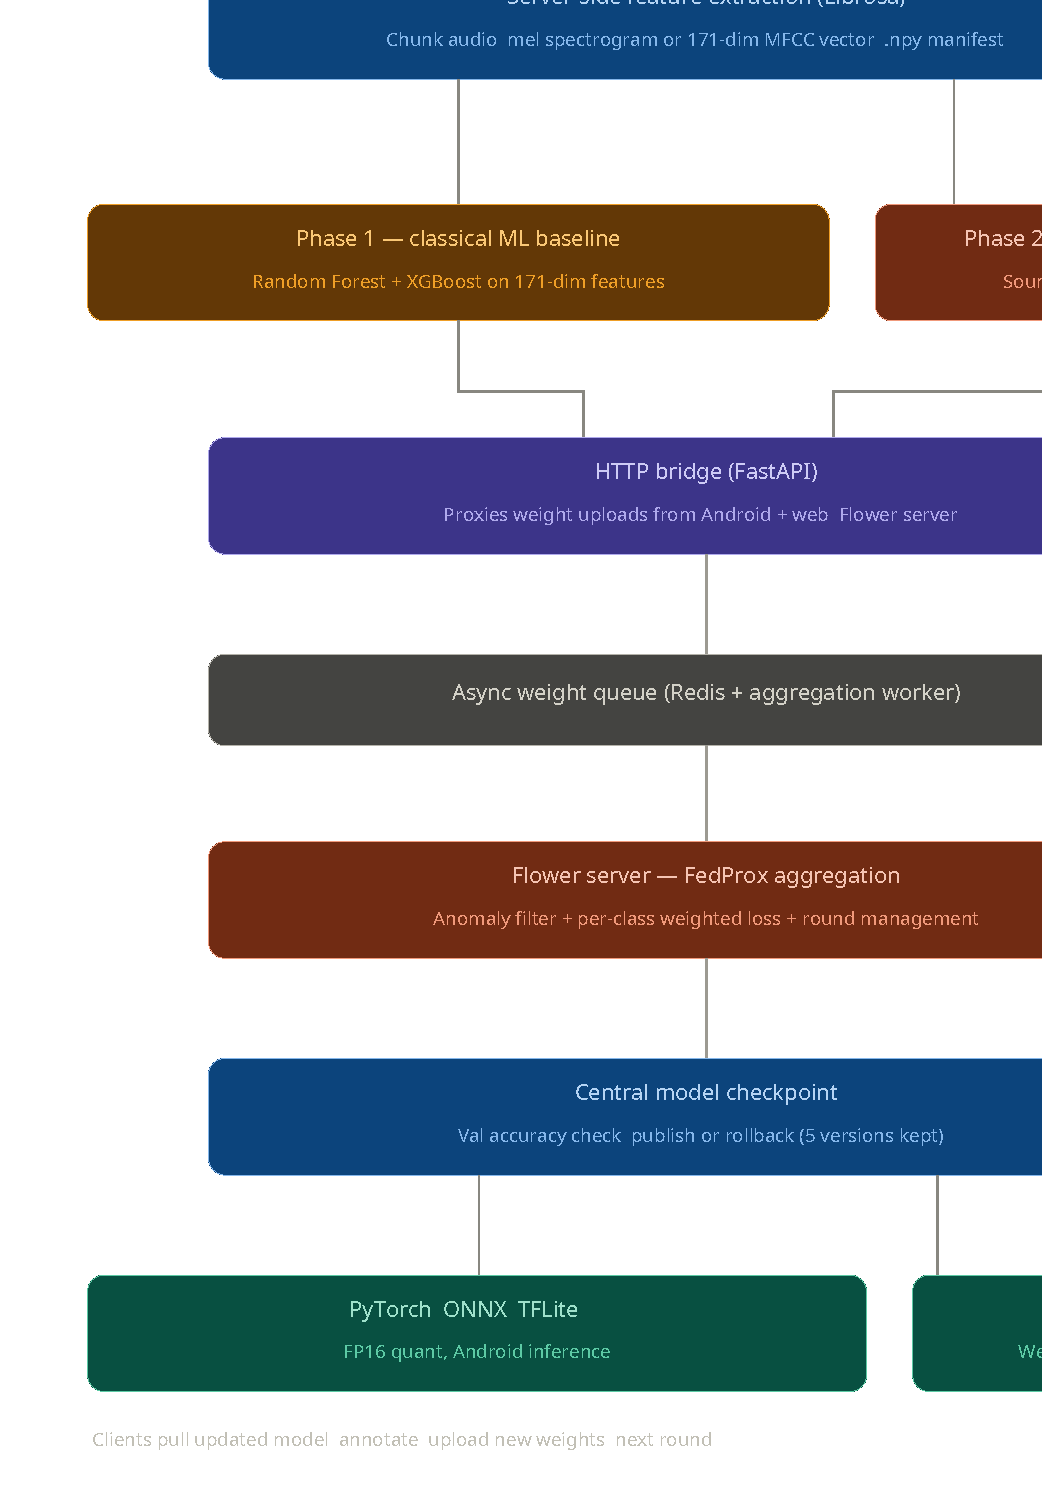
\includegraphics[width=0.85\textwidth]{soundtag_fl_system_diagram_v2.pdf}
\caption{SoundTag Federated Learning System Architecture — full pipeline from edge clients through feature extraction, ML/DL training, Flower FedProx aggregation, and model export to TFLite/TF.js.}
\label{fig:system_architecture}
\end{figure}

\subsection{Framework: Flower (flwr)}

Flower is the federated learning orchestration layer. It is framework-agnostic
(PyTorch, TensorFlow, scikit-learn), supports FedAvg, FedProx, FedAdam, and
custom strategies out of the box, and handles client-server communication.

\begin{keybox}
\textbf{Important constraint.} Flower clients are Python processes. The Android
app and web browser cannot run a native Flower client. Both clients communicate
with the Flower server via a \textbf{thin HTTP bridge} (FastAPI) that proxies weight
uploads and model downloads. The bridge receives serialised NumPy weights from the
app, wraps them as a Flower \texttt{FitRes} response, and injects them into the
aggregation round. This is the canonical approach for mobile federated learning with
Flower and is fully supported.
\end{keybox}

\subsection{Server: FedProx Strategy}

FedProx is preferred over vanilla FedAvg because SoundTag clients collect
non-IID data: a user near a construction site will record mostly
\texttt{construction}, while a user in a market will record mostly \texttt{crowd}.
FedProx adds a proximal term that prevents large divergence from the global model
during local training.

\begin{lstlisting}[language=Python, caption={Flower Server with FedProx}]
import flwr as fl
from flwr.server.strategy import FedProx
import torch
from pathlib import Path

def evaluate_global(server_round: int, parameters: fl.common.NDArrays,
                    config: dict):
    """
    Called after each round. Evaluates the aggregated model on the
    central held-out validation set.
    """
    model = SoundTagCNN(num_classes=8)
    params_dict = zip(model.state_dict().keys(), parameters)
    state_dict  = {k: torch.tensor(v) for k, v in params_dict}
    model.load_state_dict(state_dict, strict=True)

    val_acc = run_validation(model, "data/val_manifest.csv",
                              "data/features_dl/")
    return float(val_acc), {"val_accuracy": float(val_acc)}


strategy = FedProx(
    proximal_mu          = 0.1,    # Proximal term strength (tune 0.01-1.0)
    fraction_fit         = 0.3,    # 30% of available clients per round
    fraction_evaluate    = 0.0,    # Evaluation done centrally, not on clients
    min_fit_clients      = 3,      # Minimum clients to start a round
    min_available_clients= 5,      # Wait until 5 clients are registered
    evaluate_fn          = evaluate_global,
    initial_parameters   = fl.common.ndarrays_to_parameters(
        [val.cpu().numpy() for val in
         SoundTagCNN(num_classes=8).state_dict().values()]
    )
)

if __name__ == "__main__":
    fl.server.start_server(
        server_address = "0.0.0.0:8080",
        config         = fl.server.ServerConfig(num_rounds=100),
        strategy       = strategy,
    )
\end{lstlisting}

\subsection{HTTP Bridge: FastAPI Weight Exchange Endpoint}

This service sits between the mobile clients and the Flower server. It receives
weight payloads from Android and web clients, queues them asynchronously, and
injects them into the active Flower aggregation round.

\begin{lstlisting}[language=Python, caption={FastAPI HTTP Bridge (Weight Exchange)}]
from fastapi import FastAPI, HTTPException, BackgroundTasks
from pydantic import BaseModel
from typing import Optional
import numpy as np
import json, uuid, time
from pathlib import Path
import asyncio
import redis.asyncio as aioredis

app   = FastAPI(title="SoundTag FL Bridge")
redis = aioredis.from_url("redis://localhost:6379")

# --- Request/Response Models ---

class WeightSubmission(BaseModel):
    client_id:    str
    round_id:     int
    num_samples:  int
    model_version:str
    weights_b64:  str    # Base64-encoded JSON list of flattened numpy arrays

class ModelInfo(BaseModel):
    version:   str
    round_id:  int
    url:       str
    size_bytes:int

# --- Endpoints ---

@app.post("/api/v1/weights/submit")
async def submit_weights(payload: WeightSubmission,
                          background_tasks: BackgroundTasks):
    """
    Receives weight update from an edge client.
    Validates, stores in Redis queue for async aggregation.
    """
    job_id = str(uuid.uuid4())
    job = {
        "job_id":       job_id,
        "client_id":    payload.client_id,
        "round_id":     payload.round_id,
        "num_samples":  payload.num_samples,
        "model_version":payload.model_version,
        "weights_b64":  payload.weights_b64,
        "received_at":  time.time(),
        "status":       "queued"
    }
    await redis.lpush("weight_queue", json.dumps(job))
    return {"job_id": job_id, "status": "queued"}


@app.get("/api/v1/weights/status/{job_id}")
async def weight_status(job_id: str):
    """Client polls this to check if their update was aggregated."""
    status = await redis.get(f"job:{job_id}:status")
    if status is None:
        raise HTTPException(404, "Job not found")
    return {"job_id": job_id, "status": status.decode()}


@app.get("/api/v1/model/latest", response_model=ModelInfo)
async def get_latest_model():
    """Returns metadata for the latest published global model."""
    info = await redis.get("model:latest:info")
    if info is None:
        raise HTTPException(503, "No global model available yet")
    return json.loads(info)


@app.get("/api/v1/model/version")
async def get_model_version():
    version = await redis.get("model:latest:version")
    return {"version": version.decode() if version else "none"}


@app.get("/api/v1/round/info")
async def get_round_info():
    info = await redis.get("round:current:info")
    return json.loads(info) if info else {"status": "idle", "round_id": 0}
\end{lstlisting}

\subsection{Aggregation Worker}

The aggregation worker runs as a separate process, draining the Redis weight
queue and triggering Flower rounds when enough updates have arrived.

\begin{lstlisting}[language=Python, caption={Asynchronous Aggregation Worker}]
import asyncio
import json
import base64
import numpy as np
import torch
import redis.asyncio as aioredis
from pathlib import Path

MIN_CLIENTS_PER_ROUND = 3
ROUND_TIMEOUT_SECONDS = 3600   # Start round after 1h even if fewer clients

async def aggregation_worker():
    r = aioredis.from_url("redis://localhost:6379")
    print("Aggregation worker started. Waiting for weight submissions...")

    while True:
        # Collect pending submissions
        pending = []
        while True:
            item = await r.rpop("weight_queue")
            if item is None:
                break
            pending.append(json.loads(item))

        if len(pending) >= MIN_CLIENTS_PER_ROUND:
            await run_aggregation_round(r, pending)
        else:
            # Re-queue and wait
            for item in pending:
                await r.lpush("weight_queue", json.dumps(item))
            await asyncio.sleep(60)   # Check every minute


async def run_aggregation_round(r, submissions: list):
    """FedProx-style weighted averaging of submitted weights."""
    print(f"Starting aggregation round with {len(submissions)} clients")

    # Deserialise all weight arrays
    client_weights = []
    total_samples  = 0
    for sub in submissions:
        raw = json.loads(base64.b64decode(sub["weights_b64"]))
        arrays = [np.array(a, dtype=np.float32) for a in raw]
        client_weights.append((arrays, sub["num_samples"]))
        total_samples += sub["num_samples"]

    # Weighted average (FedAvg / FedProx shares the same aggregation step)
    n_layers = len(client_weights[0][0])
    global_weights = []
    for layer_idx in range(n_layers):
        layer_avg = sum(
            w[layer_idx] * (n / total_samples)
            for w, n in client_weights
        )
        global_weights.append(layer_avg)

    # Load into model and evaluate
    model = SoundTagCNN(num_classes=8)
    state_dict = {k: torch.tensor(v)
                  for k, v in zip(model.state_dict().keys(), global_weights)}
    model.load_state_dict(state_dict, strict=True)

    val_acc = run_validation(model, "data/val_manifest.csv",
                              "data/features_dl/")

    # Increment round counter; save model if improved
    round_id   = int(await r.incr("round:counter"))
    prev_best  = float(await r.get("model:best_val_acc") or 0.0)

    if val_acc > prev_best:
        version = f"v{round_id}"
        save_path = Path(f"models/global/{version}.pt")
        save_path.parent.mkdir(parents=True, exist_ok=True)
        torch.save(model.state_dict(), save_path)

        await r.set("model:best_val_acc", str(val_acc))
        await r.set("model:latest:version", version)
        info = {"version": version, "round_id": round_id,
                "url": f"/models/{version}.pt",
                "size_bytes": save_path.stat().st_size}
        await r.set("model:latest:info", json.dumps(info))
        print(f"  -> Round {round_id}: New best model published "
              f"(val_acc={val_acc:.4f})")
    else:
        print(f"  -> Round {round_id}: No improvement "
              f"(val_acc={val_acc:.4f} <= best={prev_best:.4f}), "
              f"global model unchanged")

    # Mark jobs as aggregated
    for sub in submissions:
        await r.set(f"job:{sub['job_id']}:status", "aggregated", ex=86400)


if __name__ == "__main__":
    asyncio.run(aggregation_worker())
\end{lstlisting}

\subsection{Edge Client: Android (Local Fine-Tuning + Weight Upload)}

On Android, the TFLite model handles inference. Local fine-tuning is performed
by a lightweight Python-in-Java environment (Chaquopy) or, more practically,
by a separate on-device training loop using \textbf{TensorFlow Lite Model
Personalisation API} (which supports gradient updates without Chaquopy).

\begin{lstlisting}[language=C, caption={Android FL Client (Kotlin)}]
// FLClient.kt
class FLClient(
    private val context: Context,
    private val annotatorId: String,
    private val serverUrl: String
) {
    private var modelVersion: String = "none"
    private val localSamples: MutableList<Pair<FloatArray, Int>> = mutableListOf()

    // ---- Step 1: Pull latest global model ----
    suspend fun checkAndDownloadModel() {
        val response = withContext(Dispatchers.IO) {
            URL("$serverUrl/api/v1/model/version").readText()
        }
        val serverVersion = JSONObject(response).getString("version")
        if (serverVersion != modelVersion) {
            downloadModel(serverVersion)
            modelVersion = serverVersion
        }
    }

    private suspend fun downloadModel(version: String) {
        // Download .tflite file and save to internal storage
        val modelUrl  = "$serverUrl/models/$version.tflite"
        val modelFile = File(context.filesDir, "soundtag_model.tflite")
        withContext(Dispatchers.IO) {
            URL(modelUrl).openStream().use { input ->
                modelFile.outputStream().use { output -> input.copyTo(output) }
            }
        }
        Log.d("FLClient", "Downloaded model $version")
    }

    // ---- Step 2: Store a locally annotated sample ----
    fun addLocalSample(melFeatures: FloatArray, label: Int) {
        localSamples.add(Pair(melFeatures, label))
    }

    // ---- Step 3: Fine-tune and upload when enough samples ----
    suspend fun fineTuneAndUpload(minSamples: Int = 10) {
        if (localSamples.size < minSamples) return

        // Fine-tuning is done via the TFLite Task Audio personalisation API
        // or a simple gradient step using the Flower Android SDK.
        // Here we serialise the current model weights and the local data
        // and send them to the server for server-side aggregation.

        val modelFile   = File(context.filesDir, "soundtag_model.tflite")
        val weightBytes = modelFile.readBytes()
        val weightB64   = Base64.encodeToString(weightBytes, Base64.NO_WRAP)

        val payload = JSONObject().apply {
            put("client_id",     annotatorId)
            put("round_id",      0)   // Server resolves current round
            put("num_samples",   localSamples.size)
            put("model_version", modelVersion)
            put("weights_b64",   weightB64)
        }

        withContext(Dispatchers.IO) {
            val url  = URL("$serverUrl/api/v1/weights/submit")
            val conn = url.openConnection() as HttpURLConnection
            conn.requestMethod = "POST"
            conn.setRequestProperty("Content-Type", "application/json")
            conn.doOutput = true
            conn.outputStream.write(payload.toString().toByteArray())
            val code = conn.responseCode
            Log.d("FLClient", "Weight upload response: $code")
        }

        localSamples.clear()
    }
}
\end{lstlisting}

\subsection{Edge Client: Web (TF.js + Weight Upload)}

\begin{lstlisting}[language=Python, caption={Web FL Client (TypeScript)}]
// fl_client.ts
import * as tf from '@tensorflow/tfjs';

const CLASSES = [
  'traffic','horn','construction','industrial',
  'crowd','nature','silence','mixed'
];

export class WebFLClient {
  private model:        tf.LayersModel | null = null;
  private modelVersion: string = 'none';
  private localSamples: { mel: tf.Tensor; label: number }[] = [];
  private readonly serverUrl: string;
  private readonly clientId:  string;

  constructor(serverUrl: string, clientId: string) {
    this.serverUrl = serverUrl;
    this.clientId  = clientId;
  }

  // Pull latest model if version changed
  async checkAndLoadModel(): Promise<void> {
    const res     = await fetch(`${this.serverUrl}/api/v1/model/version`);
    const { version } = await res.json();
    if (version !== this.modelVersion) {
      const info = await (await fetch(`${this.serverUrl}/api/v1/model/latest`)).json();
      this.model        = await tf.loadLayersModel(info.url);
      this.modelVersion = version;
      console.log(`[FLClient] Loaded model ${version}`);
    }
  }

  // Run inference on a mel spectrogram tensor
  async predict(melTensor: tf.Tensor3D): Promise<{ label: string; confidence: number }> {
    if (!this.model) await this.checkAndLoadModel();
    const input  = melTensor.expandDims(0);          // (1,1,128,T)
    const logits = this.model!.predict(input) as tf.Tensor;
    const probs  = logits.softmax().arraySync() as number[][];
    const p      = probs[0];
    const top    = p.indexOf(Math.max(...p));
    return { label: CLASSES[top], confidence: p[top] };
  }

  // Store a locally confirmed sample for federated contribution
  addSample(melTensor: tf.Tensor3D, label: number): void {
    this.localSamples.push({ mel: melTensor.clone(), label });
  }

  // Upload current weights to the FL server
  async uploadWeights(): Promise<void> {
    if (!this.model || this.localSamples.length < 5) return;

    const weights   = this.model.getWeights();
    const weightData = await Promise.all(
      weights.map(async (w) => Array.from(await w.data()))
    );
    const weightsB64 = btoa(JSON.stringify(weightData));

    const payload = {
      client_id:     this.clientId,
      round_id:      0,
      num_samples:   this.localSamples.length,
      model_version: this.modelVersion,
      weights_b64:   weightsB64,
    };

    const res = await fetch(`${this.serverUrl}/api/v1/weights/submit`, {
      method:  'POST',
      headers: { 'Content-Type': 'application/json' },
      body:    JSON.stringify(payload),
    });
    const { job_id } = await res.json();
    console.log(`[FLClient] Weight upload queued. Job ID: ${job_id}`);

    // Dispose tensors and clear samples
    this.localSamples.forEach(s => s.mel.dispose());
    this.localSamples = [];
  }
}
\end{lstlisting}

% ============================================================
\section{Model Export: From PyTorch to Edge Formats}
% ============================================================

Once the central model achieves acceptable validation accuracy, it is exported
to TFLite (Android) and TF.js (web) for deployment as the edge inference model.

\begin{lstlisting}[language=Python, caption={Model Export Pipeline (PyTorch -> ONNX -> TFLite + TF.js)}]
import torch
import onnx
import subprocess
from pathlib import Path

def export_to_onnx(model_pt_path: str, onnx_path: str,
                    input_shape=(1, 1, 128, 215)):
    """Export PyTorch model to ONNX."""
    model = SoundTagCNN(num_classes=8)
    model.load_state_dict(torch.load(model_pt_path, map_location="cpu"))
    model.eval()

    dummy_input = torch.randn(*input_shape)
    torch.onnx.export(
        model, dummy_input, onnx_path,
        export_params=True,
        opset_version=12,
        do_constant_folding=True,
        input_names=["mel_spectrogram"],
        output_names=["logits"],
        dynamic_axes={"mel_spectrogram": {0: "batch_size"}}
    )
    onnx.checker.check_model(onnx.load(onnx_path))
    print(f"Exported to ONNX: {onnx_path}")


def export_to_tflite(onnx_path: str, tflite_path: str,
                      quantize: bool = True):
    """Convert ONNX -> TFLite via tf2onnx + TFLiteConverter."""
    # Step 1: ONNX -> TF SavedModel
    saved_model_dir = onnx_path.replace(".onnx", "_savedmodel")
    subprocess.run([
        "python", "-m", "tf2onnx.convert",
        "--onnx", onnx_path,
        "--output", saved_model_dir,
        "--saved-model"
    ], check=True)

    # Step 2: SavedModel -> TFLite
    import tensorflow as tf
    converter = tf.lite.TFLiteConverter.from_saved_model(saved_model_dir)
    if quantize:
        converter.optimizations = [tf.lite.Optimize.DEFAULT]
        converter.target_spec.supported_types = [tf.float16]
    tflite_model = converter.convert()
    Path(tflite_path).write_bytes(tflite_model)
    print(f"Exported to TFLite: {tflite_path} "
          f"({Path(tflite_path).stat().st_size / 1024:.0f} KB)")


def export_to_tfjs(saved_model_dir: str, tfjs_dir: str):
    """Convert TF SavedModel -> TF.js for web deployment."""
    subprocess.run([
        "tensorflowjs_converter",
        "--input_format=tf_saved_model",
        "--output_node_names=logits",
        "--saved_model_tags=serve",
        saved_model_dir, tfjs_dir
    ], check=True)
    print(f"Exported to TF.js: {tfjs_dir}")
\end{lstlisting}

% ============================================================
\section{Infrastructure and Deployment}
% ============================================================

\subsection{Server Stack}

\begin{table}[h]
\centering
\caption{Recommended Server Configuration}
\begin{tabular}{@{}p{4cm}p{8cm}@{}}
\toprule
\textbf{Component} & \textbf{Specification} \\
\midrule
GPU (training) & NVIDIA L4 (24 GB) or T4 (16 GB) on RunPod/Vast.ai \\
CPU & 8 vCPUs (AMD EPYC or Xeon) \\
RAM & 32 GB system RAM \\
Storage & 200 GB NVMe SSD \\
Network & 1 Gbps \\
OS & Ubuntu 22.04 LTS \\
\bottomrule
\end{tabular}
\end{table}

\textbf{Note on GPU sizing.} At 50 annotators and a 650K-parameter model,
an L4 at \$0.60/h (RunPod spot) or T4 at \$0.35/h is sufficient.
An A100 is unnecessary until the model exceeds 10M parameters or the
dataset exceeds 500K samples. Scale up then, not now.

\subsection{Docker Compose}

\begin{lstlisting}[language=bash, caption={docker-compose.yml}]
version: "3.9"
services:

  fl_server:
    build: .
    image: soundtag-fl:latest
    command: python fl_server.py
    ports: ["8080:8080"]
    volumes: ["./models:/app/models", "./data:/app/data"]
    deploy:
      resources:
        reservations:
          devices: [{driver: nvidia, count: 1, capabilities: [gpu]}]

  api:
    image: soundtag-fl:latest
    command: uvicorn bridge:app --host 0.0.0.0 --port 8000 --workers 4
    ports: ["8000:8000"]
    depends_on: [redis]
    environment:
      - REDIS_URL=redis://redis:6379

  worker:
    image: soundtag-fl:latest
    command: python aggregation_worker.py
    depends_on: [redis]
    volumes: ["./models:/app/models", "./data:/app/data"]
    deploy:
      resources:
        reservations:
          devices: [{driver: nvidia, count: 1, capabilities: [gpu]}]

  redis:
    image: redis:7-alpine
    volumes: ["redis_data:/data"]
    command: redis-server --appendonly yes

  postgres:
    image: postgres:16-alpine
    environment:
      POSTGRES_DB:       soundtag
      POSTGRES_USER:     soundtag
      POSTGRES_PASSWORD: ${DB_PASSWORD}
    volumes: ["pg_data:/var/lib/postgresql/data"]

volumes:
  redis_data:
  pg_data:
\end{lstlisting}

\subsection{Python Dependencies}

\begin{lstlisting}[language=bash, caption={requirements.txt}]
# Core ML
torch==2.3.0
torchvision==0.18.0
librosa==0.10.2
numpy==1.26.4
scikit-learn==1.4.2
pandas==2.2.2
tqdm==4.66.4
joblib==1.4.2

# Federated learning
flwr[simulation]==1.8.0

# API and queue
fastapi==0.111.0
uvicorn[standard]==0.30.1
redis[asyncio]==5.0.4
pydantic==2.7.3

# Model export
onnx==1.16.1
onnxruntime==1.18.0
tf2onnx==1.16.1
tensorflow==2.16.1
tensorflowjs==4.19.0
\end{lstlisting}

% ============================================================
\section{Dataset Requirements and Collection Timeline}
% ============================================================

\subsection{Minimum Viable Thresholds}

\begin{table}[h]
\centering
\caption{Dataset Size Thresholds}
\begin{tabular}{@{}p{4cm}p{3cm}p{3cm}p{3.5cm}@{}}
\toprule
\textbf{Phase} & \textbf{Per Class} & \textbf{Total Samples} & \textbf{Purpose} \\
\midrule
ML baseline   & 200  & 1,600  & Classical model + pipeline validation \\
DL initial    & 500  & 4,000  & First CNN training run \\
DL solid      & 2,000 & 16,000 & Reliable cross-validation \\
FL production & 5,000 & 40,000 & Federated rounds with 10+ annotators \\
\bottomrule
\end{tabular}
\end{table}

\subsection{Diversity Requirements}

For the model to generalise beyond the recording conditions of a few users:

\begin{itemize}[leftmargin=*,noitemsep]
  \item \textbf{Geographic:} At least 10 distinct locations (different neighbourhoods,
        not just different streets in one area)
  \item \textbf{Temporal:} Recordings across all four time bands: morning rush (7--9~AM),
        midday (11~AM--1~PM), evening rush (5--7~PM), and night (10~PM--12~AM)
  \item \textbf{Device:} At least 5 different device models (microphone response
        varies significantly across manufacturers)
  \item \textbf{Annotator:} At least 3 annotators per class (reduces individual
        perception bias)
\end{itemize}

\subsection{Phased Collection Plan}

\begin{table}[h]
\centering
\caption{Phased Data Collection Timeline}
\begin{tabular}{@{}p{2.5cm}p{2.5cm}p{7cm}@{}}
\toprule
\textbf{Phase} & \textbf{Target} & \textbf{Strategy} \\
\midrule
Week 1--2  & 1,600 samples  & 4 annotators, 50 clips/day each, all 8 classes balanced \\
Week 3--4  & 4,000 samples  & Expand to 8 annotators; focus on underrepresented classes \\
Week 5--8  & 10,000 samples & 15+ annotators; crowdsource via public beta \\
Week 9+    & Continuous     & FL rounds every time 3+ annotators submit updates \\
\bottomrule
\end{tabular}
\end{table}

% ============================================================
\section{Federated Round Protocol}
% ============================================================

\subsection{Round Trigger Conditions}

A new federated round is triggered when \textbf{any} of the following is true:

\begin{itemize}[leftmargin=*,noitemsep]
  \item $\geq 3$ client weight submissions are queued, \textbf{or}
  \item 6 hours have elapsed since the last round with $\geq 1$ submission queued
\end{itemize}

\subsection{Round Execution Sequence}

\begin{enumerate}[leftmargin=*,noitemsep]
  \item Aggregation worker wakes, pops all pending submissions from the Redis queue
  \item Checks anomaly filter: reject submissions whose mean weight norm deviates
        $> 3\sigma$ from the median across submissions in this round
  \item Runs weighted FedProx averaging (Algorithm 1)
  \item Evaluates aggregated model on central validation set
  \item If $\Delta\text{acc} > 0$, increments model version, saves checkpoint,
        publishes to \texttt{model:latest:info} in Redis
  \item If $\Delta\text{acc} \leq 0$, retains previous model and logs the failed round
  \item Marks all contributing job IDs as \texttt{aggregated}
\end{enumerate}

\subsection{Anomaly Filter (Adversarial Robustness)}

\begin{lstlisting}[language=Python, caption={Weight Anomaly Filter}]
def filter_anomalous_submissions(submissions: list,
                                  sigma_threshold: float = 3.0) -> list:
    """
    Rejects submissions whose L2 norm of flattened weights is an outlier.
    Protects against Byzantine clients sending corrupted or adversarial updates.
    """
    norms = []
    for sub in submissions:
        raw = json.loads(base64.b64decode(sub["weights_b64"]))
        flat = np.concatenate([np.array(a).flatten() for a in raw])
        norms.append(np.linalg.norm(flat))

    norms = np.array(norms)
    median = np.median(norms)
    mad    = np.median(np.abs(norms - median))

    filtered = []
    for sub, norm in zip(submissions, norms):
        z = (norm - median) / (mad + 1e-8)
        if abs(z) <= sigma_threshold:
            filtered.append(sub)
        else:
            print(f"  [Filter] Rejected client {sub['client_id']}: "
                  f"weight norm z={z:.2f}")
    return filtered
\end{lstlisting}

% ============================================================
\section{Monitoring and Metrics}
% ============================================================

Track the following per round and store in PostgreSQL:

\begin{table}[h]
\centering
\caption{Metrics to Track}
\begin{tabular}{@{}p{4cm}p{8cm}@{}}
\toprule
\textbf{Metric} & \textbf{Purpose} \\
\midrule
Per-class F1 score & Overall accuracy hides class-level failures \\
Validation loss per round & Detect overfitting or divergence \\
Client participation rate & How many registered annotators contributed this round \\
Weight norm distribution & Inputs to anomaly filter; early signal of drift \\
Correction rate (inference) & How often users override the model's prediction \\
Class distribution per client & Detect data skew across geographic areas \\
\bottomrule
\end{tabular}
\end{table}

\textbf{Alert conditions.}
Trigger an operator alert if: (1) validation accuracy drops $> 2\%$ from the
previous round, (2) fewer than 1 client contributes in a 72-hour window, or
(3) any class F1 drops below 0.4 for two consecutive rounds.

% ============================================================
\section{Risk and Mitigation}
% ============================================================

\begin{table}[h]
\centering
\caption{Risk Register}
\begin{tabular}{@{}p{3.5cm}p{4cm}p{5cm}@{}}
\toprule
\textbf{Risk} & \textbf{Impact} & \textbf{Mitigation} \\
\midrule
Non-IID data across clients & Model favours majority classes & FedProx + weighted sampling + per-class loss weights \\
Class imbalance & Poor recall on rare classes & WeightedRandomSampler; oversample centrally \\
Feature inconsistency (SR mismatch) & Training/inference mismatch & All feature extraction on server; versioned pipeline config \\
Model regression after aggregation & Worse global model deployed & Keep last 5 checkpoints; automatic rollback if val\_acc drops \\
Low client participation & Stale global model & Round timeout trigger; reduce min\_fit\_clients floor \\
Adversarial weight submission & Corrupted global model & Weight norm anomaly filter (z-score, $3\sigma$) \\
Network failure during upload & Lost weight update & Redis queue with persistent AOF; client retries with job ID \\
\bottomrule
\end{tabular}
\end{table}

% ============================================================
\section{Publication Roadmap}
% ============================================================

\subsection{Suggested Venue Targets}

\begin{itemize}[leftmargin=*,noitemsep]
  \item \textbf{Primary:} IEEE Transactions on Audio, Speech, and Language Processing;
        or INTERSPEECH (audio classification + FL methodology)
  \item \textbf{Secondary:} ACM BuildSys (urban sensing + mobile systems angle);
        or ICLR workshop on FL in the Wild
  \item \textbf{Dataset paper:} Scientific Data (Nature) if the SoundTag corpus
        reaches $\geq 10{,}000$ samples across $\geq 5$ cities
\end{itemize}

\subsection{Contribution Claims (Differentiators)}

\begin{enumerate}[leftmargin=*,noitemsep]
  \item A \textbf{purpose-built urban noise corpus} (SoundTag) with GPS, temporal
        metadata, and multi-severity annotations from real-world mobile collection
  \item A \textbf{two-phase modelling methodology}: handcrafted ML features as a
        reproducible baseline, followed by a custom CNN/CRNN trained from scratch
  \item A \textbf{practical FL deployment} on heterogeneous edge devices
        (Android + web browser) using an HTTP bridge architecture that resolves the
        Flower native-client limitation for mobile environments
  \item An \textbf{async weight queue} (Redis-backed) enabling FL in intermittent
        mobile network conditions, with Byzantine-robust anomaly filtering
  \item Empirical results on \textbf{non-IID urban noise data} under FedProx,
        including per-class F1 analysis across geographic client clusters
\end{enumerate}

\subsection{Experimental Sections Required for Publication}

\begin{enumerate}[leftmargin=*,noitemsep]
  \item Corpus statistics: class distribution, geographic spread, annotator count,
        device diversity
  \item ML baseline: per-class F1 for Random Forest and XGBoost, confusion matrix
  \item DL from scratch: SoundTagCNN vs SoundTagCRNN, ablation on augmentation
  \item Federated learning: FedAvg vs FedProx; convergence curves; non-IID
        performance gap vs. centralised training
  \item Efficiency analysis: communication cost per round (bytes), inference
        latency on target devices (Android mid-range, browser), model size
\end{enumerate}

% ============================================================
\section{Implementation Roadmap}
% ============================================================

\begin{table}[h]
\centering
\caption{Week-by-Week Implementation Plan}
\begin{tabular}{@{}p{2cm}p{3.5cm}p{7cm}@{}}
\toprule
\textbf{Week} & \textbf{Milestone} & \textbf{Deliverable} \\
\midrule
1   & Data pipeline & \texttt{build\_dataset()} validated; manifest CSV; first 1,600 samples \\
1--2 & ML baseline & RF + XGBoost trained; cross-validation results; confusion matrix \\
2--3 & DL pipeline & SoundTagCNN and CRNN training; val accuracy $>$ ML baseline \\
3   & Server setup & Docker Compose up; Redis + PostgreSQL running; FastAPI endpoints live \\
4   & Model export & PyTorch $\to$ ONNX $\to$ TFLite (Android) + TF.js (web) \\
4--5 & Android client & TFLite inference working; weight upload to HTTP bridge \\
5   & Web client & TF.js inference working; weight upload to HTTP bridge \\
6   & FL first round & 3+ annotators contributing; first aggregation round completes \\
7--8 & Monitoring & Per-class F1 dashboard; anomaly filter logs; rollback tested \\
9+  & Scale + paper & 10,000+ samples; run experiments; write Sections 4--6 of paper \\
\bottomrule
\end{tabular}
\end{table}

% ============================================================
\section{Conclusion}
% ============================================================

This document defines a complete, reproducible framework for training an urban
noise classification model via federated learning. The architecture prioritises:

\begin{itemize}[leftmargin=*,noitemsep]
  \item \textbf{Data pipeline correctness} over premature accuracy optimisation.
        A versioned, single-point extraction pipeline ensures that every model
        trained on SoundTag data uses identical features.
  \item \textbf{Practical FL deployment.} The HTTP bridge pattern resolves the
        real constraint that Flower does not support native browser or Android
        clients, without sacrificing the aggregation logic or server-side tooling.
  \item \textbf{Progressive complexity.} Classical ML first, then CNN, then CRNN.
        Each phase validates the previous and provides publication-ready ablation
        results.
  \item \textbf{Publication readiness.} The combination of a novel annotated
        corpus, a from-scratch DL methodology, and a mobile FL deployment on
        heterogeneous devices constitutes a complete and differentiable research
        contribution.
\end{itemize}

The automatic on-device annotation (showing model predictions to users for
confirmation) is a natural inference by-product of the deployment step and
requires no additional ML development---it is simply the forward pass of the
exported edge model.

\vspace{1cm}
\noindent\rule{\textwidth}{0.5pt}
\noindent\textbf{Document version:} 2.0 \\
\noindent\textbf{Date:} \today \\
\noindent\textbf{Author:} SoundTag ML Team \\
\noindent\textbf{Status:} Ready for implementation

\end{document}